%-------------------------
% Resume in Latex
% Author : Javier Tarazona
%------------------------

\documentclass[letterpaper,10pt]{article}
\DeclareUnicodeCharacter{00A0}{~}
\DeclareUnicodeCharacter{2013}{\textendash}
\DeclareUnicodeCharacter{2014}{\textemdash}
\DeclareUnicodeCharacter{201C}{``}
\DeclareUnicodeCharacter{201D}{''}
\DeclareUnicodeCharacter{2022}{\textbullet}
\DeclareUnicodeCharacter{25E6}{\textopenbullet}
% \setlist[itemize]{label=\textbullet, labelsep=0.5em, leftmargin=*} % Moved after \begin{document}
\usepackage[T1]{fontenc}
\usepackage[empty]{fullpage}
\usepackage[export]{adjustbox}
\usepackage[pdftex]{hyperref}
\usepackage[usenames,dvipsnames]{color}
\usepackage[utf8]{inputenc}
\usepackage{array}
\usepackage{comment}
\usepackage{enumitem}
\usepackage{enumitem}
\usepackage{fancyhdr}
\usepackage{graphicx}
\usepackage{latexsym}
\usepackage{lmodern}
\usepackage{marvosym}
\usepackage{tabularx}
\usepackage{titlesec}
\usepackage{verbatim}
\usepackage{xcolor}


\usepackage{latexsym}
\usepackage[empty]{fullpage}
\usepackage{titlesec}
\usepackage{marvosym}
\usepackage[usenames,dvipsnames]{color}
\usepackage{verbatim}
\usepackage{enumitem}
\usepackage[pdftex]{hyperref}
\usepackage{fancyhdr}
\usepackage{tabularx}
\usepackage{graphicx}
\usepackage{array}
\usepackage[export]{adjustbox}
\usepackage{xcolor}
\usepackage{comment}

\begin{comment}
\end{comment}
% --- Safe encoding and fonts ---
\usepackage[utf8]{inputenc}
\usepackage[T1]{fontenc}
\usepackage{enumitem}

% --- Clean and safe bullets ---
\setlist[itemize]{label=\textbullet, labelsep=0.5em, leftmargin=*}
%\end{comment}

\pagestyle{empty}

% Adjust margins
\addtolength{\oddsidemargin}{-0.45in}
\addtolength{\evensidemargin}{-0.45in}
\addtolength{\textwidth}{1.15in}
\addtolength{\topmargin}{-.62in}
\addtolength{\textheight}{1.20in}

\urlstyle{same}

\raggedbottom
\raggedright
\setlength{\tabcolsep}{0in}
\renewcommand{\arraystretch}{0.98}

%\definecolor{mydarkgreen}{RGB}{0, 140, 123}
\definecolor{mydarkgreen}{RGB}{0, 0, 0}

% Sections formatting
\titleformat{\section}{
  \vspace{-5pt}\scshape\raggedright\large
}{}{0em}{}[\color{mydarkgreen}\titlerule \vspace{-6pt}]

%-------------------------
% Custom commands
\newcommand{\resumeItemCompact}[2]{\item\small{\textbf{#1}: #2}\vspace{-2pt}}
\newcommand{\resumeItemListStartCompact}{\begin{itemize}[leftmargin=*,itemsep=0pt,parsep=0pt,topsep=0pt,partopsep=0pt,nolistsep]}
\newcommand{\resumeItemListEndCompact}{\end{itemize}\vspace{-4pt}}

\newcommand{\resumeItem}[2]{
  \item\small{
    \textbf{#1}{: #2 \vspace{-2pt}}
  }
}

\newcommand{\resumeSubheading}[4]{
  \vspace{-1pt}\item
    \begin{tabular*}{0.97\textwidth}{l@{\extracolsep{\fill}}r}
      	\textbf{#1} & \textbf{\textcolor{mydarkgreen}{#2}} \\
      	\textit{\footnotesize#3} & \textit{\footnotesize \textcolor{mydarkgreen}{#4}} \\
    \end{tabular*}\vspace{-4pt}
}

\newcommand{\resumeSubItem}[2]{\resumeItem{#1}{#2}\vspace{-4pt}}

\renewcommand{\labelitemii}{$\circ$}

\newcommand{\resumeSubHeadingListStart}{\begin{itemize}[leftmargin=*]}
\newcommand{\resumeSubHeadingListEnd}{\end{itemize}}
\newcommand{\resumeItemListStart}{\begin{itemize}[itemsep=0pt,parsep=0pt,topsep=0pt,partopsep=0pt]}
\newcommand{\resumeItemListEnd}{\end{itemize}\vspace{-5pt}}

% Indented paragraph helper: \indentbox[width]{content}
\newcommand{\indentbox}[2][1em]{\hspace*{#1}\parbox{\dimexpr\linewidth-#1\relax}{#2}}

\newlength{\headerPhotoSpace}
\setlength{\headerPhotoSpace}{0pt}
\newcommand{\showHeaderPhoto}{%
  \setlength{\headerPhotoSpace}{0.13\textwidth}%
  \makebox[0pt][l]{\adjustbox{valign=c}{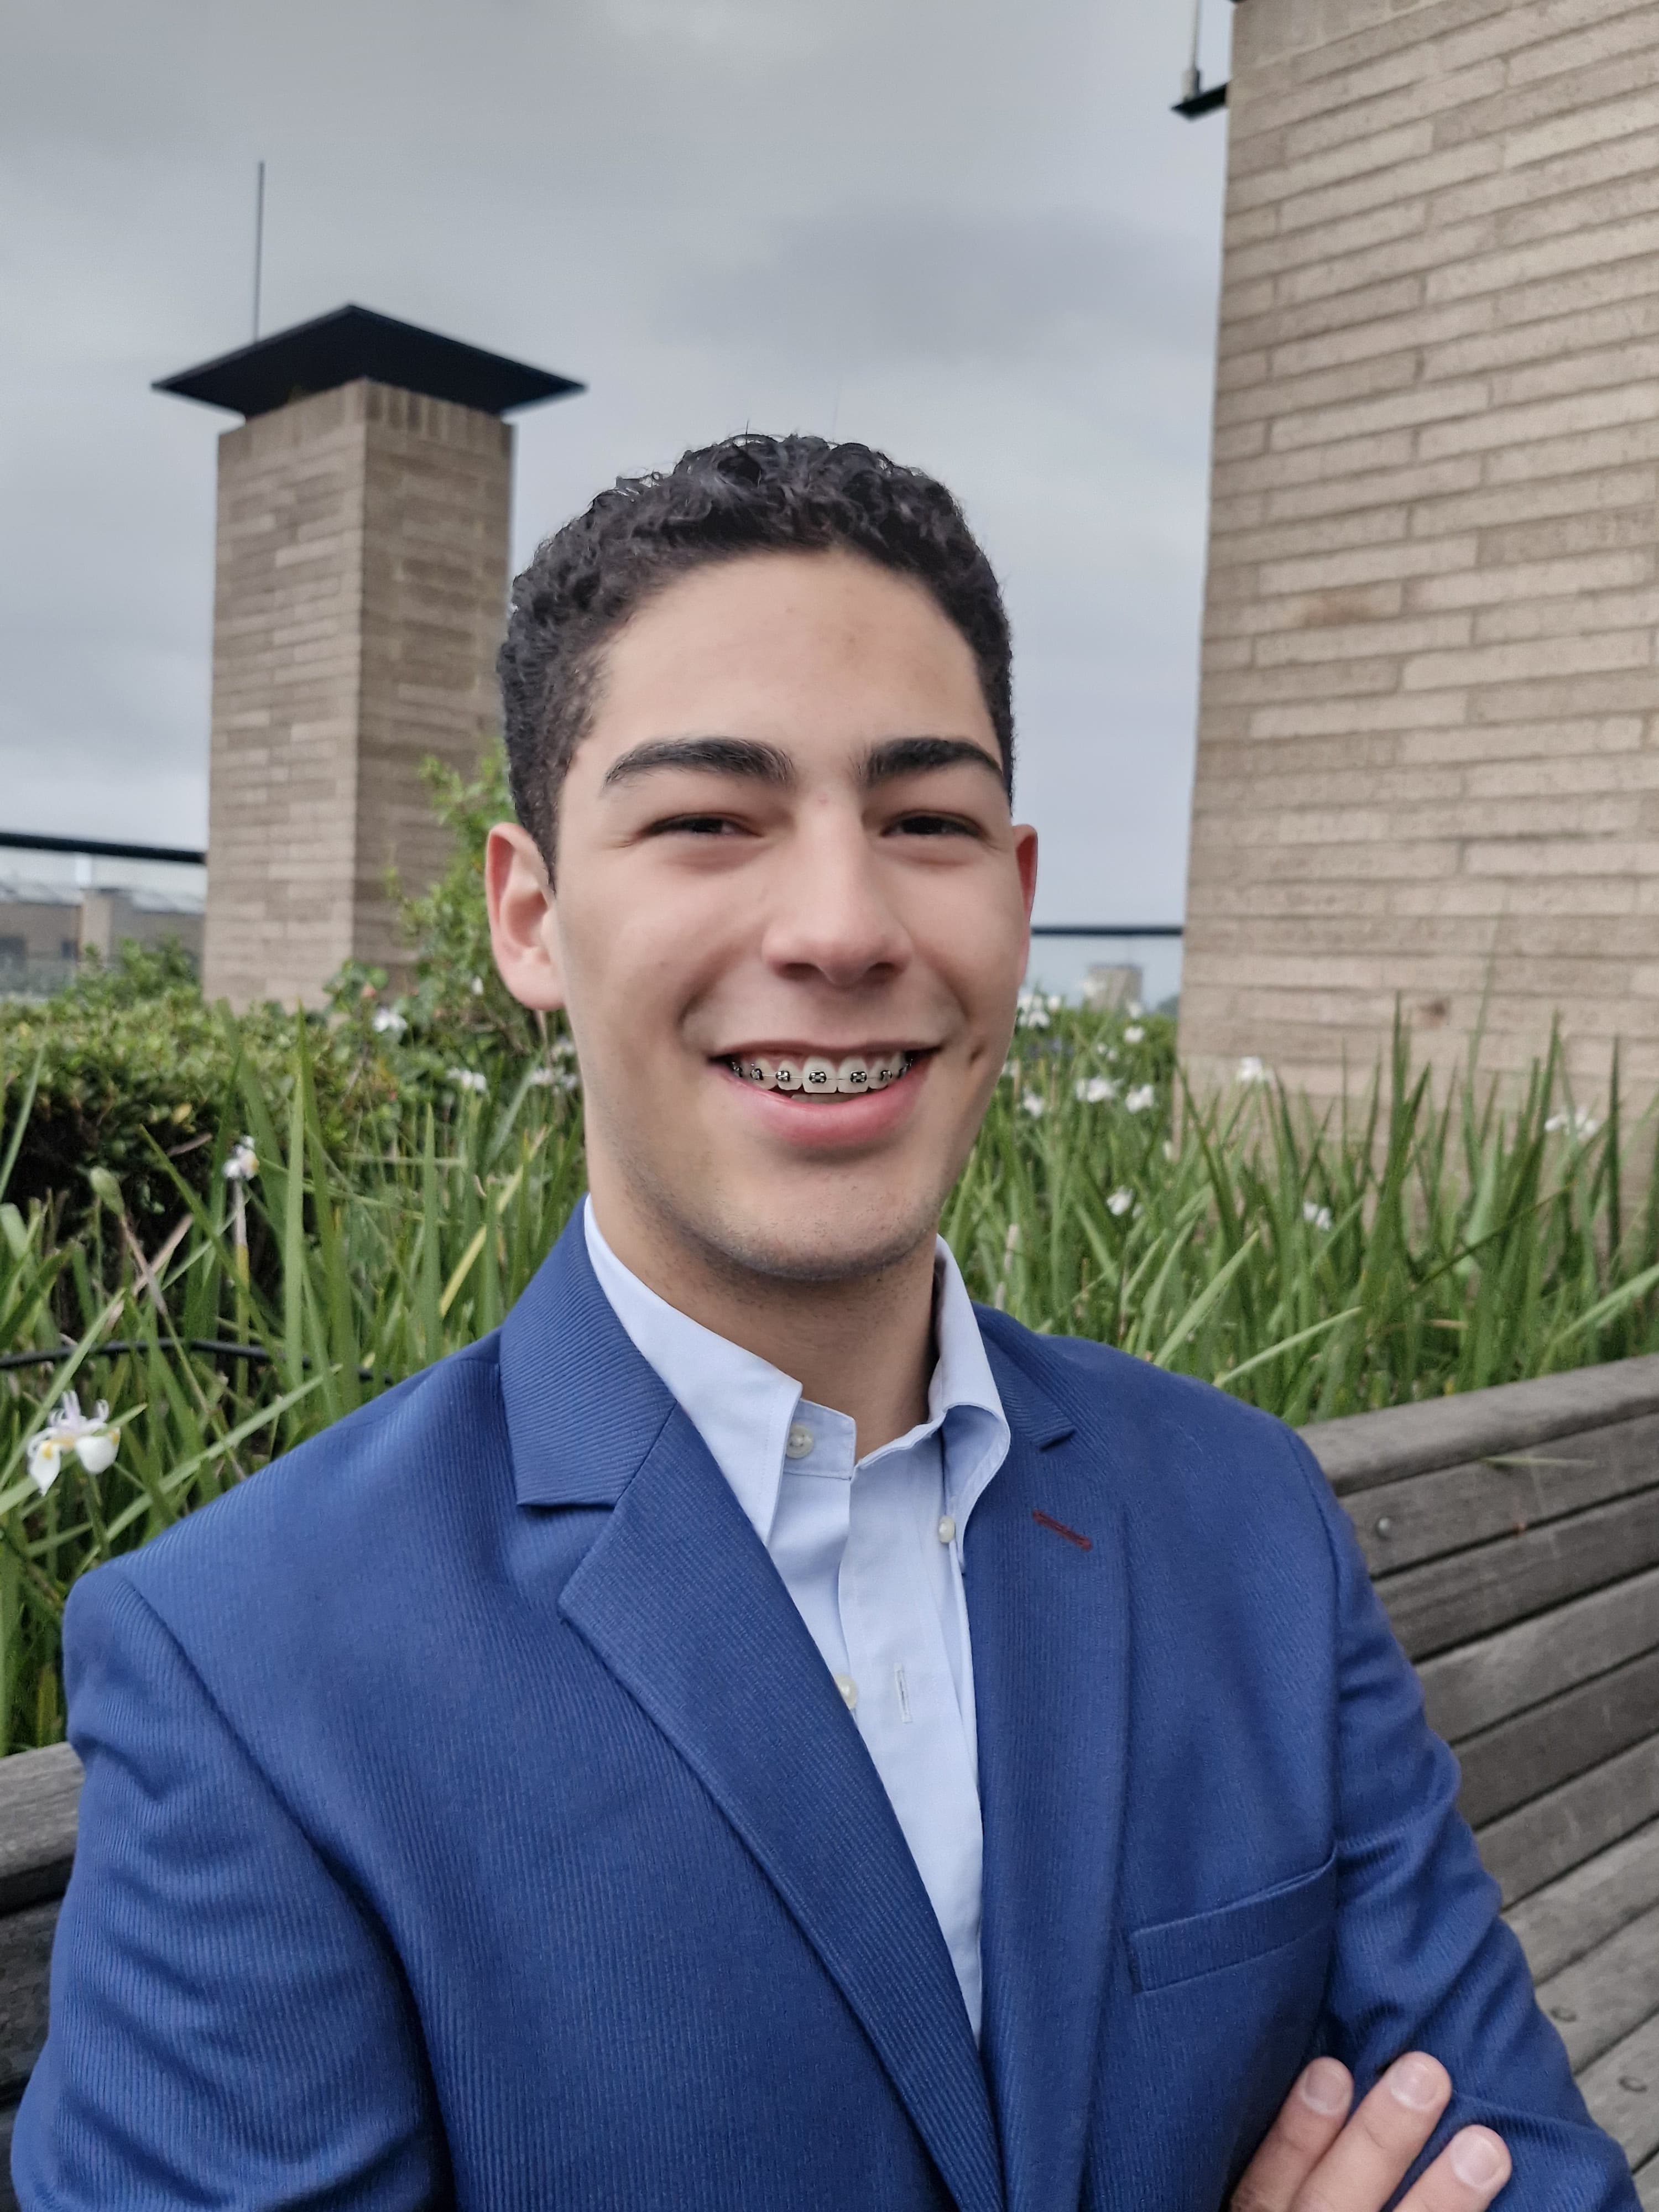
\includegraphics[scale=0.015]{Digital_photo.jpg}}}%
}


%-------------------------------------------
%%%%%%  CV STARTS HERE  %%%%%%%%%%%%%%%%%%%%%%%%%%%%


\begin{document}

% QR Code----------------

\begin{comment}
\AddToHookNext{shipout/foreground}{%
  \put(\dimexpr\paperwidth-0.35cm\relax,-\dimexpr\paperheight-0.35cm\relax){%
    \makebox(0,0)[rb]{%
      \begin{minipage}{2.25cm}
        \centering
        {\setlength{\fboxsep}{1pt}\colorbox{white}{%
          \parbox{2.0cm}{\centering\scriptsize\bfseries Scan QR code\\[-1pt]for digital version}}}\\[1pt]
        
\includegraphics[width=1.6cm]{qr_CV.png}%
      \end{minipage}%
    }%
  }%
}
\end{comment}

% --- Clean and safe bullets ---
\setlist[itemize]{label=\textbullet, labelsep=0.5em, leftmargin=*}

%----------HEADING-----------------

\noindent
\showHeaderPhoto% Comment this line to remove the photo and expand the header.
\hspace*{\headerPhotoSpace}%
\begin{minipage}[c]{\dimexpr\textwidth-\headerPhotoSpace\relax}
  \begin{tabular*}{\linewidth}{@{}l@{\extracolsep{\fill}}r@{}}

            \textbf{\Large \textcolor{mydarkgreen}{Javier Andrés TARAZONA JIMENEZ}} & \textbf{\textcolor{mydarkgreen}{Email:}} \href{mailto:javitar06@gmail.com}{javitar06@gmail.com}\\

            \footnotesize Student - Systems and Computer Engineer - Artificial Intelligence & \href{mailto:javier-andres.tarazona@ensta-paris.fr}{javier-andres.tarazona@ensta-paris.fr}\\

            \href{https://www.linkedin.com/in/javier-andres-tarazona-jimenez-84b489222/}{\textcolor{blue}{\underline{LinkedIn}}} & \textbf{\textcolor{mydarkgreen}{Mobile:}} +33 07 46 36 97 75 \\

            \href{https://github.com/JavierTarazona06}{\textcolor{blue}{\underline{GitHub}}} & Paris, France\\
        \end{tabular*}
\end{minipage}

\vspace{0.3cm}

%\textbf{Seeking a final-year work-study position in artificial intelligence, from in September 2026}
\textbf{Seeking a 5 to 6 months internship in artificial intelligence, from in September 2026}

\vspace{-0.05cm}

%-----------EDUCATION-----------------
\section{\textcolor{mydarkgreen}{\textbf{EDUCATION}}}

\begin{tabularx}{\textwidth}{>{\raggedright\arraybackslash}X >{\raggedleft\arraybackslash}p{0.24\textwidth}}
  \begin{minipage}[t]{\linewidth}\raggedright
  \textbullet\ \textbf{Institut Polytechnique de Paris (IPP) - ENSTA}\\
  \textit{\footnotesize 2nd engineering school in France (L'Etudiant 2026); IPP ranked 41st worldwide (QS 2026)}\\
  \textit{\footnotesize Master of Science in Engineering - AI Track}\\
  \textit{\footnotesize Relevant coursework: Machine Learning, Statistics, Image recognition, Neurocomputational models}
  \end{minipage}
  &
  \begin{minipage}[t]{\linewidth}\raggedleft
  \textbf{Paris, France}\\
  {\footnotesize\textit{September 2025 -- Present}}
  \end{minipage}
  \\
  \begin{minipage}[t]{\linewidth}
  \textbullet\ \textbf{Universidad Nacional de Colombia (UNAL)}\\
  \textit{\footnotesize 12th in Latin America (QS Latin America 2026)}\\
  \textit{\footnotesize Systems and Computer Engineering}\\
  \textit{\footnotesize Relevant coursework: Multi-Agent Systems, Stochastic Models, Optimization}
  \end{minipage}
  &
  \begin{minipage}[t]{\linewidth}\raggedleft
  \textbf{Bogotá, Colombia}\\
  {\footnotesize\textit{January 2021 -- July 2025}}
  \end{minipage}
  \\
  \begin{minipage}[t]{\linewidth}
  \textbullet\ \textbf{University of Saskatchewan}\\
  \textit{\footnotesize Academic exchange.}\\
  \textit{\footnotesize Coursework: Software Engineering, Algorithms, Operating Systems and Business French}
  \end{minipage}
  &
  \begin{minipage}[t]{\linewidth}\raggedleft
  \textbf{Saskatoon, Canada}\\
  {\footnotesize\textit{September 2024 -- December 2024}}
  \end{minipage}
\end{tabularx}

\vspace{0.1cm}
%--------AWARDS------------
\section{\textcolor{mydarkgreen}{\textbf{AWARDS}}}

\begin{tabularx}{\textwidth}{
  % Width sum: 0.75 + 1.45 + 0.80 = 3.00
  >{\hsize=0.75\hsize\linewidth=\hsize\raggedright\arraybackslash}X
  >{\hsize=1.48\hsize\linewidth=\hsize\raggedright\arraybackslash}X
  >{\hsize=0.70\hsize\linewidth=\hsize\raggedright\arraybackslash}X}
    \begin{minipage}[t]{\linewidth}\raggedright
      \textbullet\ \textbf{\textbf{Eiffel Excellence Scholarship}}\\
      \textit{\footnotesize ENSTA - Master 2025\textendash{}2027}\\
    \end{minipage}
    &
    \begin{minipage}[t]{\linewidth}\raggedright
      \textbullet\ \textbf{Honorable Mention \textendash{} ICPC Colombia 2023}\\
      {\footnotesize\textit{XXXVII National Programming Marathon ACIS REDIS}}
    \end{minipage}
    &
    \begin{minipage}[t]{\linewidth}\raggedright
      \textbullet\ \textbf{Academic Excellence}\\
      {\footnotesize\textit{UNAL - Tuition waiver}}
    \end{minipage}\\
\end{tabularx}


\vspace{0.1cm}
%-----------EXPERIENCE-----------------
\section{\textcolor{mydarkgreen}{\textbf{PROFESSIONAL EXPERIENCE}}}
  \begin{tabularx}{\textwidth}{>{\raggedright\arraybackslash}X >{\raggedleft\arraybackslash}p{0.4\textwidth}}


    \begin{minipage}[t]{\linewidth}\raggedright
      \textbullet\ \textbf{ENSTA Paris -- U2IS}\\
      \textit{\footnotesize Research Intern in Artificial Intelligence and 3D Vision}\\
    \end{minipage}
    &
    \begin{minipage}[t]{\linewidth}\raggedleft
      \textbf{Palaiseau, France}\\
      {\footnotesize\textit{May 2026 -- Present}}
    \end{minipage}\\

    \multicolumn{2}{l}{
      \begin{minipage}[t]{\linewidth}\raggedright
        \indentbox{\footnotesize \textbf{- Self-supervised 3D vision: } Novel view synthesis on a synthetic 3D dataset of progressively complex geometric shapes (\textbf{curriculum learning}).}
      \end{minipage}
    }\\

    \multicolumn{2}{l}{
      \begin{minipage}[t]{\linewidth}\raggedright
        \indentbox{\footnotesize \textbf{- 3D data generation with Blender: } \textbf{Python/Blender} pipeline for multi-view rendering, cameras, metadata and training-data organization.}
      \end{minipage}
    }\\

    \multicolumn{2}{l}{
      \begin{minipage}[t]{\linewidth}\raggedright
        \indentbox{\footnotesize \textbf{- Deep Learning: } Pre-training through novel-view prediction with \textbf{PyTorch} and \textbf{Vision Transformers} to learn 3D structure.}
      \end{minipage}
    }\\

    %------------------------------------

    \begin{minipage}[t]{\linewidth}\raggedright
      \textbullet\ \textbf{APEDYS91}\\
      \textit{\footnotesize Machine Learning / NLP Engineer}\\
    \end{minipage}
    &
    \begin{minipage}[t]{\linewidth}\raggedleft
      \textbf{Paris, France}\\
      {\footnotesize\textit{October 2025 - February 2026}}
    \end{minipage}\\

    \multicolumn{2}{l}{
    \begin{minipage}[t]{\linewidth}\raggedright
        \indentbox{\footnotesize \textbf{- AI and NLP Development: } Local French text correction application based on a \textbf{rules \& LLMs pipeline} (LanguageTool, Mistral/Gemma), with spaCy NER guardrails, entity/number checks and RAM/VRAM-based model selection.}
    \end{minipage}
    }\\

    %------------------------------------
    %------------------------------------

    \begin{minipage}[t]{\linewidth}\raggedright
      \textbullet\ \textbf{Engin A.I}\\
      \textit{\footnotesize Software and Computer Vision Engineer}\\
    \end{minipage}
    &
    \begin{minipage}[t]{\linewidth}\raggedleft
      \textbf{Colombia - United States}\\
      {\footnotesize\textit{12 months: Jan. - Jul. 2024 and Feb. - Jun. 2025}}
    \end{minipage}\\

    \multicolumn{2}{l}{
      \begin{minipage}[t]{\linewidth}\raggedright
        \indentbox{\footnotesize \textbf{- Python refactoring: } Refactoring of two libraries into an object-oriented, modular architecture; \textbf{+70 \% refactoring score} based on maintainability index, duplication, test coverage, lines of code and cyclomatic complexity.}
      \end{minipage}
    }\\

    \multicolumn{2}{l}{
      \begin{minipage}[t]{\linewidth}\raggedright
        \indentbox{\footnotesize \textbf{- Computer Vision (OpenCV, NumPy, Mathematics): }Optimization of lane/road-marking post-processing (\textbf{+50 \% speed, +60 \% accuracy}) and WheelPath trajectory generation to correlate deterioration areas.}
      \end{minipage}
    }\\


  \end{tabularx}


\vspace{0.1cm}
%%------------------------------
%%------------------------------
%%------------------------------
\section{\textcolor{mydarkgreen}{\textbf{ACADEMIC PROJECTS}}}

  \begin{tabularx}{\textwidth}{>{\raggedright\arraybackslash}X >{\raggedleft\arraybackslash}p{0.01\textwidth}}

    \begin{minipage}[t]{\linewidth}\raggedright
      \textbullet\ \textbf{"Tameo" - Embedded vision for an autonomous system (ongoing project)}\\
      \textit{\footnotesize Python, PyTorch, YOLO, ZED, DWA, supervised learning, detection/segmentation}\\
      \indentbox{\footnotesize Vision pipeline for detection and movement-decision support on an autonomous boat; fine-tuning on specialized datasets, data augmentation and model benchmarking, improving mAP, F1 and precision/recall from about 80\% to 90\%.}\\
    \end{minipage}
    &
    \begin{minipage}[t]{\linewidth}\raggedleft %Text here
    \end{minipage}\\

    \begin{minipage}[t]{\linewidth}\raggedright
      \textbullet\ \textbf{Slow - Traffic video analyzer}\\
      \textit{\footnotesize Python, Tkinter, OpenCV, MySQL, PyMySQL, Matplotlib, Pillow}\\
      \indentbox{\footnotesize Vehicle tracking and speed estimation from traffic videos with OpenCV; Tkinter/MySQL interface and Matplotlib reports. \href{https://github.com/JavierTarazona06/slow}{\textcolor{blue}{\underline{More information}}}.}\\
    \end{minipage}
    &
    \begin{minipage}[t]{\linewidth}\raggedleft %Text here
    \end{minipage}\\

    \begin{minipage}[t]{\linewidth}\raggedright
      \textbullet\ \textbf{Skin segmentation with statistical learning - Computer Vision}\\
      \textit{\footnotesize Python, OpenCV, NumPy, scikit-learn, K-Means, Gaussian Naive Bayes, QDA, RGB/HSV/YCrCb}\\
      \indentbox{\footnotesize Pixel-wise segmentation pipeline for face images: RGB/HSV/YCrCb feature extraction and Cb-Cr descriptors enriched with luminance gradients, then benchmarking Gaussian Naive Bayes, QDA and K-Means to generate skin masks. \href{https://github.com/JavierTarazona06/Vision_LocalFeatures_BayesianClassification_KMeans/blob/main/docs/rappport/rap.pdf}{\textcolor{blue}{\underline{More information}}}.}
    \end{minipage}
    &
    \begin{minipage}[t]{\linewidth}\raggedleft %Text here
    \end{minipage}\\

  \end{tabularx}




%--------EXPERTISE------------
%\section{\textcolor{mydarkgreen}{\textbf{p}}}

\vspace{4pt}
\noindent\rule{\textwidth}{0.4pt}
\vspace{0.4pt}

% Keep each heading in the same minipage as its list to preserve PDF text extraction order.
\noindent
\begin{minipage}[t]{0.60\textwidth}
  \raggedright
  \textbf{\underline{Technical Skills}}\\[-2pt]
  {\scriptsize
    \begin{itemize}[leftmargin=*,itemsep=1pt,parsep=0pt,topsep=0pt,partopsep=0pt]
      \item \textbf{AI tools:} Python, PyTorch, OpenCV, NumPy, Pandas, spaCy, LanguageTool, Llama, Vision Transformers, Blender/Python API
      \item \textbf{Programming, Software and Cloud:} Google Cloud Platform (GCP), Docker, Django, FastAPI,
        React, JavaScript, C++/C, Java, SQL/NoSQL, Windows packaging and distribution (PyInstaller, Inno Setup)
      \item \textbf{Methodologies:} Agile (SCRUM), Git/GitHub, CI/CD, software architecture
    \end{itemize}
  }

  \vspace{0.15cm}
  \textbf{\underline{Soft Skills}}\\[-2pt]
  {\scriptsize
    \begin{itemize}[leftmargin=*,itemsep=1pt,parsep=0pt,topsep=0pt,partopsep=0pt]
      \item Leadership
      \item Cross-cultural communication
    \end{itemize}
  }
\end{minipage}\hfill
\begin{minipage}[t]{0.36\textwidth}
  \raggedright
  \textbf{\underline{Languages}}\\[-2pt]
  {\scriptsize
    \begin{itemize}[leftmargin=*,itemsep=0pt,parsep=0pt,topsep=0pt,partopsep=0pt]
      \item \textbf{English} (C1 \textendash{} IELTS 2024)
      \item \textbf{French} (B2 \textendash{} DELF 2024)
      \item \textbf{Spanish} (native)
      \item \textbf{Portuguese} (basic)
    \end{itemize}
  }
\end{minipage}



%-------------------------------------------
\end{document}
